\subsection{Encontrando $\alpha$ y $\beta$}

Previamente a la experimentación nos detuvimos a analizar la fórmula que determina el RTO en una
retransimisión dada (Ver sección métodos).
$\alpha$ es utilizada para ponderar el valor de los RTT's anteriores con el último recibido.
De la ecuación para calcular el SRTT podemos deducir que valores de $\alpha$ peque\~nos hacen que
se le asigne mayor peso a las mediciones anteriores, mientras que valores de $\alpha$ mayores
establecen una mayor influencia de la última muestra de RTT obtenida.
Ambas opciones tienen ventajas y desventajas: la primera genera un RTT más estable, aunque no es
lo suficientemente rápida como para adaptarse a los cambios. La segunda aproximación es buena en
este último aspecto, aunque es susceptible a ser afectada en gran medida por fluctuaciones
temporales.

La variable $\beta$ utilizada para actualizar el valor de RTTVAR
juega un papel totalmente análogo al de $\alpha$. Valores peque\~nos hacen que se pondere en
mayor medida el valor de las variaciones anteriores, mientras que valores altos le asignan
mayor importancia al valor de la última diferencia entre la muestra del RTT obtenida y el valor
del SRTT.

Todas las mediciones destinadas a encontrar valores adecuados de $\alpha$ y $\beta$ se realizaron
con valores constantes de DELAY: 0.4 ms, probabilidad de PÉRDIDA: 0.02, K=4 y valor de
TICK\_CLOCK = 1ms

\begin{figure}[H]
  \begin{center}
      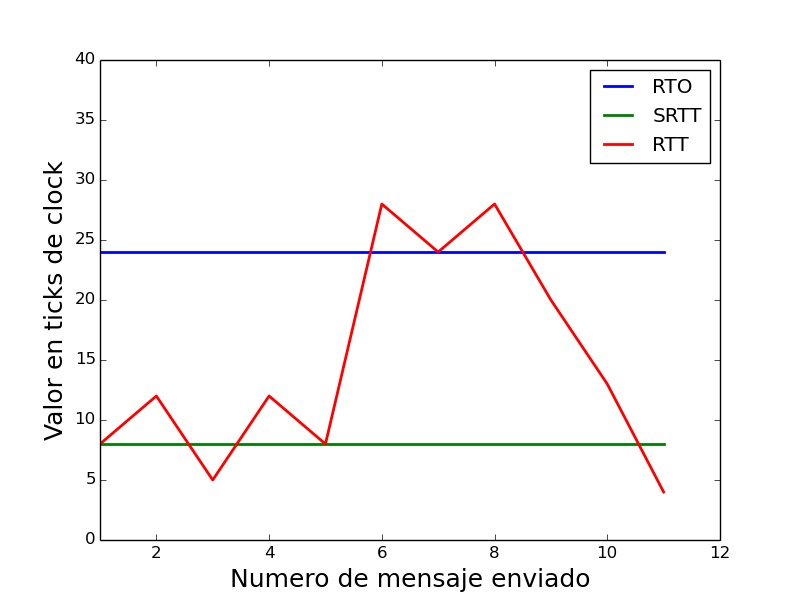
\includegraphics[scale=0.32]{imagenes/ALPHA_0_BETA_0.jpg}
      \caption{RTO, SRTT y RTT para ALPHA=0 y BETA=0}
  \end{center}
\end{figure}

Tal como puede esperarse, tomando $\alpha=0$, $\beta=0$ los cálculos ignoran por completo los nuevos
valores de RTT y consideran únicamente los valores de SRTT anteriores. En este caso, el valor constante
inicial.

\begin{figure}[H]
  \begin{center}
      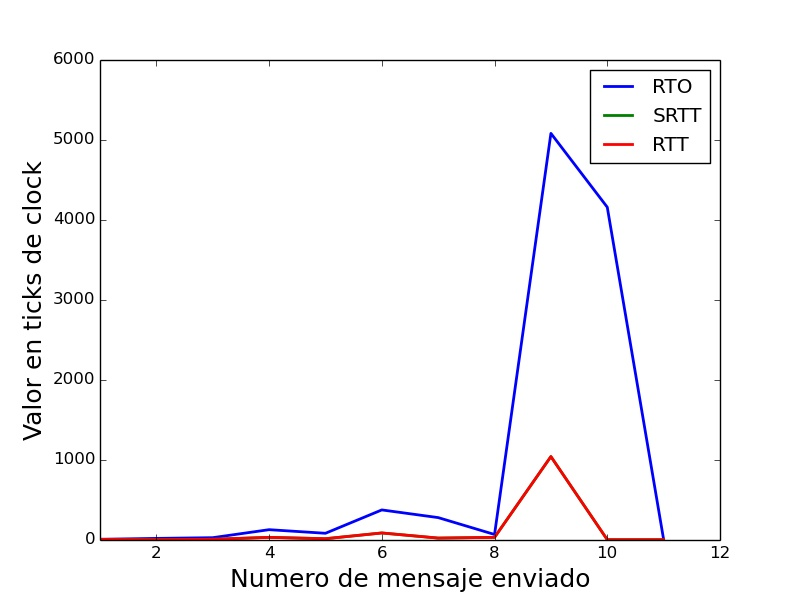
\includegraphics[scale=0.32]{imagenes/ALPHA_1_BETA_1.jpg}
      \caption{RTO, SRTT y RTT para ALPHA=1 y BETA=1}
  \end{center}
\end{figure}

Este experimento es completamente opuesto al anterior. Tomando ambas variables como 1, los cálculos
ignoran los valores anteriores (tanto de variación de RTT (RTTVAR) somo de SRTT), y modifican
los resultados únicamente en función de la última muestra de RTT obtenida. El resultado es un gráfico
en donde el RTO coincide exactamente con el SRTT, y ambos responden excesivamente a cualquier fluctuación
que se produzca en el valor del RTT.


\begin{figure}[H]
  \begin{center}
      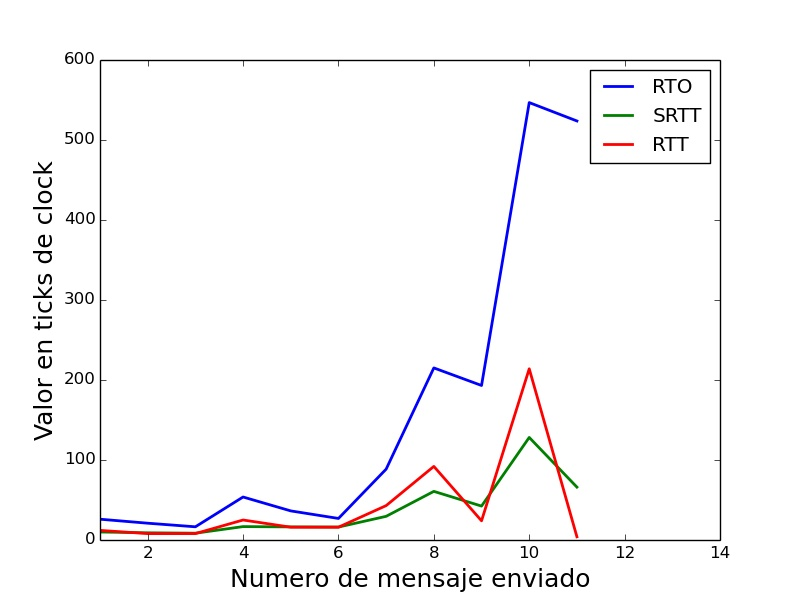
\includegraphics[scale=0.32]{imagenes/ALPHA_050_BETA_050.jpg}
      \caption{RTO, SRTT y RTT para ALPHA=0.5 y BETA=0.5}
  \end{center}
\end{figure}

Una de las primeras ideas que tuvimos fue
ponderar de igual manera los valores anteriores con los nuevos, al tomar ambas variables con valor
0.5. Esto debería generar valores cercanos a los de lasmuestras anteriores, pero que sean capaces
de responder a cambios significativos y permanentes del valor de RTT. En otras palabras, que alcancen
un equilibrio entre ambas propuestas. Sin embargo, el comportamiento no fue el esperado.
El resultado es una serie de cálculos demasiado sensibles a las fluctuaciones temporales que responden
excesivamente a estos cambios.

\begin{figure}[H]
  \begin{center}
      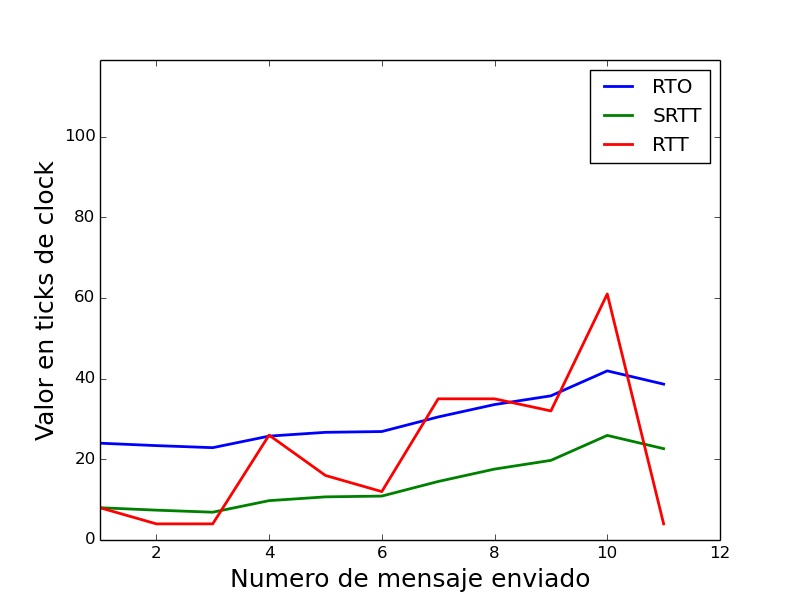
\includegraphics[scale=0.32]{imagenes/ALPHA_015_BETA_0.jpg}
      \caption{RTO, SRTT y RTT para ALPHA=0.15 y BETA=0}
  \end{center}
\end{figure}

Habiendo convalidado las hipótesis anteriores nos parece razonable fijar el valor de $\alpha$ en 0.15 (
cercano al propuesto por el RFC 6298). Las conexiones en las distintas redes por lo general permanecen
estables la mayor parte del tiempo (con lo cual la probabilidad de que el rtt permanezca inalterable
es alta), y los cambios considerables en el valor del round-trip-time son más esporádicos. De cualquier
manera, dejamos una ventana considerable para que cualquier cambio significativo en el RTT impacte
en los cálculos del SRTT. Es notorio el hecho de que el RTO aproxima bastante bien la curva del RTT, pero
lo hace de forma suave, a diferencia de esta última.

\begin{figure}[H]
  \begin{center}
      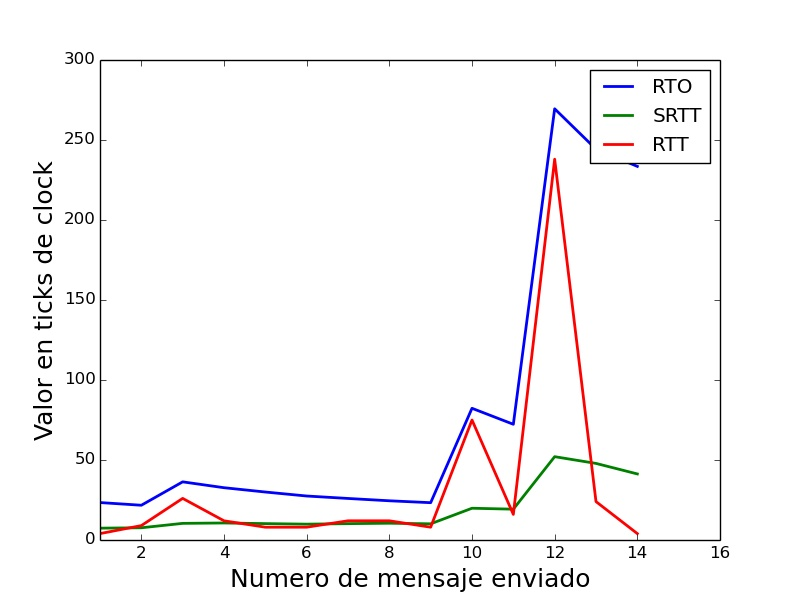
\includegraphics[scale=0.32]{imagenes/ALPHA_015_BETA_020.jpg}
      \caption{RTO, SRTT y RTT para ALPHA=0.15 y BETA=0.20}
  \end{center}
\end{figure}

Estos valores hacen que el algoritmo calcule valores mucho más cercanos a los RTT reales, a diferencia
del anterior. Ambos cambios repentinos en los valores del RTT (vistos en el gráfico como picos) son
correctamente advertidos por el cálculo del RTO. Esto se debe a que el valor de BETA cambia de 0 a
0.2, con lo cual se le agrega un poco más de sensibilidad a los cambios en el valor de los RTT's.

\begin{figure}[H]
  \begin{center}
      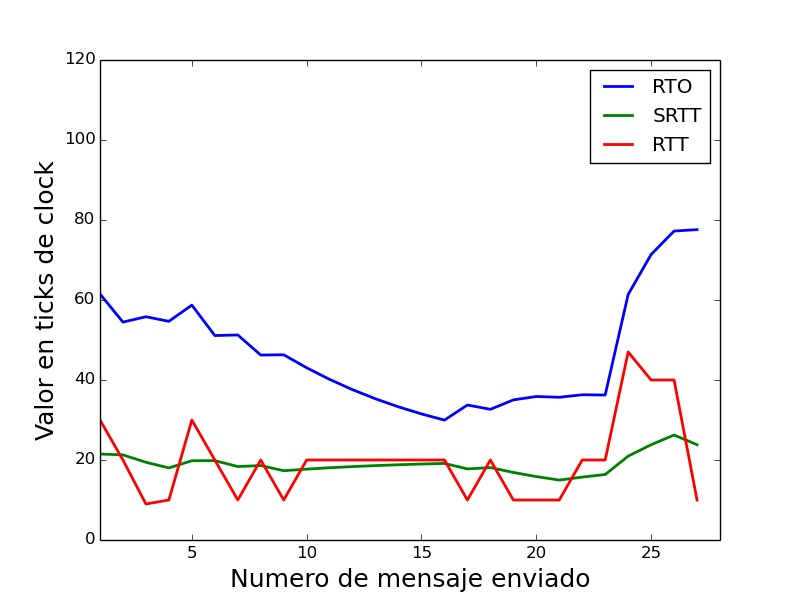
\includegraphics[scale=0.32]{imagenes/OPTIMOS_MARCO_REAL.jpg}
      \caption{RTO, SRTT y RTT para ALPHA=0.15 y BETA=0.20 en un marco real}
  \end{center}
\end{figure}

Finalmente agregamos un experimento en donde observamos el comportamiento de las actualizaciones en
un marco más real. Establecemos el valor de probabilidad de pérdida en 0.05 y el valor del delay en
10 ms.
Los valores de las variables seleccionadas se comportan realmente bien. Por un lado responden de manera
sensible a los cambios en el valor de los RTT. En suma, cuando no se
producen este tipo de cambios (situaciones hipotéticas en donde no se caigan nodos dentro de la red, o
la misma no se encuentre congestionada), el algoritmo pondera los valores anteriores y de a poco
converge al valor del RTT real.

Por estos motivos, decidimos seleccionar los valores de $\alpha=0.15$ y $\beta=0.20$.







